\documentclass[12pt]{article}
\usepackage{graphicx}
\usepackage[utf8]{inputenc}
\usepackage{amsmath}
\usepackage[top=20mm,bottom=21mm,left = 30mm , right = 30mm]{geometry}
\usepackage{xcolor}
\usepackage{wrapfig}
\usepackage{caption,subcaption}
\usepackage{hyperref}
\hypersetup{colorlinks,	citecolor=black, filecolor=black, linkcolor=black, urlcolor=black}
\usepackage{setspace}
\usepackage{pdfpages}
\usepackage{cite}
\graphicspath{{../Results/}}

\title{Autocorrelation in Weather}
\author{Pablo Lechon}
\date{}

\begin{document}

	\maketitle	
	\section{Introduction}
		The goal in this practical is to write an r script that helps answer the question: \textit{are temperatures of one year significantly correlated with the next year (successive years), across years in a given location?}\\
		For this, we calculate the correlation between $n - 1$ pairs of years, where $n$ is the total number of years. note that one cannot use the standard p-value calculated for a correlation coefficient, because measurements of climatic variables in successive time-points in a time series (successive seconds, minutes, hours, months, years, etc.) are \textit{not independent}.

	\section{Data}
		We first load the data with the comand \verb|load(filename, envir = globalenv())|, which consists of two columns: Year and Temperature. A quick plot to visualize these data can be seen in figure \ref{temp}\\
		\begin{figure}
			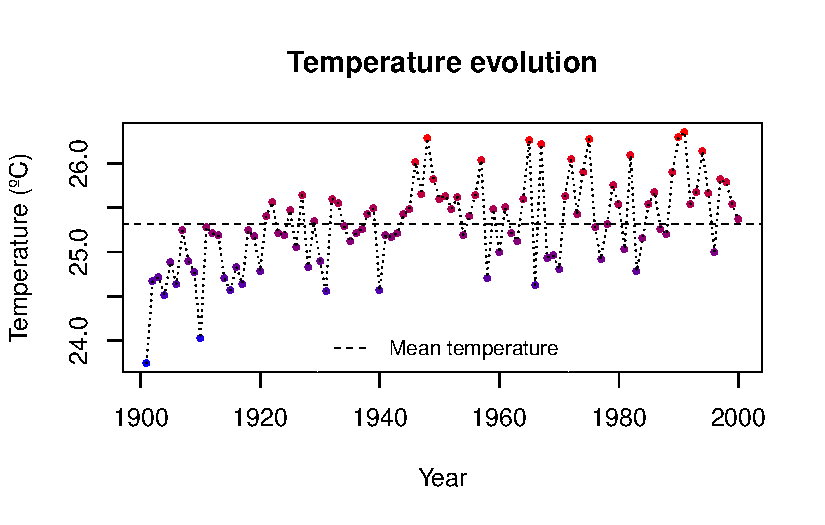
\includegraphics[width = \linewidth]{temp_evolution.pdf}	
			\centering
			\caption{Temperature time series. Redder indicates wormer. A dasshed line connects the points for better visualization. The mean temperature is represented with a horizontal dashed line}
			\label{temp}
		\end{figure}
		It can be easily seen that temperatures between consecutive years are correlated. If we calculate the correlation between consecutive years by having two Year column next to each other, shifted one position, we obtain the value 0.32. This value is meaningless if we don't determine wether or not is significant. To do it, we calculate the p-value numerically\\
	\section{p-value}
		Calculating the p-value is the same as answering the question: How likely wouldit be that, assuming no correlation between consecutive years, we obtained a value of 0.32. To calculate it numerically we make many more comparisons between two shuffled columns of years. This assures that there will be no correlation between them. We are, in fact, generating a normal distributions of correlations with mean = 0. This distribution can be seen in figure \ref{normal}\\
		\begin{figure}
			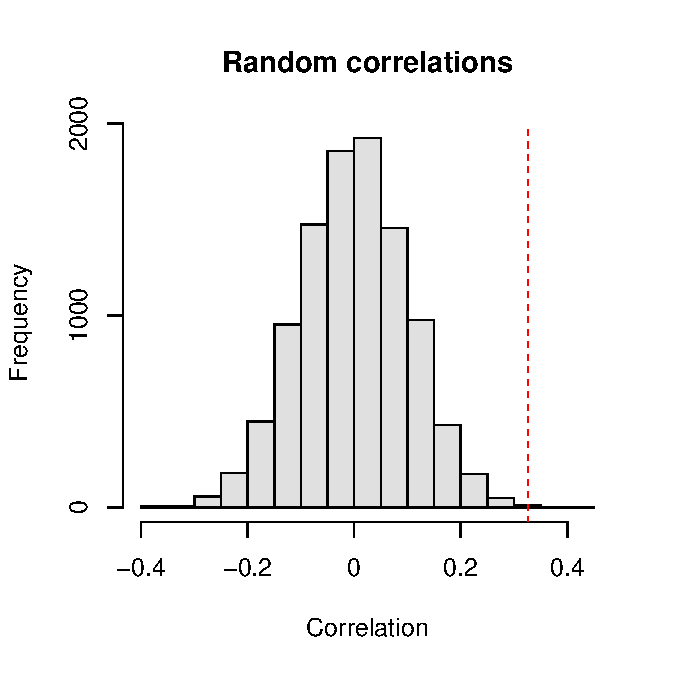
\includegraphics[scale = 0.9]{hist_p_value.pdf}
			\centering
			\caption{Normal distribution of correlation numerically generated. The vertical red line represents the correlation between consecutive years}
			\label{normal}
		\end{figure}
		To calculate the p-value we have to obtain the ratio between the correlation coefficients coming from the normal distribution that are higher than the actual correlation coefficitent. This fraction of the oreder of $10^{-4}$, wich means that the probability of finding a correlation of 0.32 by chance, is that low. Therefore, we conclude that the correlation is very significant, yet weak.
		

\end{document}
